\documentclass{article}
\usepackage{graphicx}
\usepackage{hyperref}
\usepackage[a4paper, margin=1in]{geometry}
\usepackage{breakcites}
\usepackage{subcaption}

\begin{document}

\title{Mapping Africa's Natural Safety Nets: Where Should Conservation Efforts Be Targeted to Sustain Ecosystem Services for Climate Change Resilience?}

\author{
	Cooper, Matthew\\
	%Zvoleff, Alex \\
	%Sanders, Austin \\
}

\maketitle
\begin{abstract}

In Africa, where millions of households depend on rainfed agriculture to produce food for their own consumption, climate change is a major threat to food security.  A burgeoning literature suggests that natural areas can be an asset in the face of climate change by shielding cropland from the effects of droughts, heat waves, and floods, while also providing wild foods when yields are low.  However, much of the work focusing on the "safety net" provided by forests, savannas, bodies of water and other uncultivated landcover types has been conducted in highly localized and site-specific case studies which often rely on hypothetical scenarios.  Thus, there has been little empirical and spatially explicit work on which areas provide the most benefit to local food security.  In this study, we combine data on nutrition outcomes from  300,108 children across 32 African countries with historical observations of land cover and climate shocks to test the safety net hypothesis and to map the areas that have historically played the greatest role in supporting nutrition outcomes during shocks.  These results will help conservationists to target areas providing the most benefit to local food security and nutrition, while simultaneously maximizing other conservation objectives, such as carbon sequestration and biodiversity preservation.

\end{abstract}

\section{Introduction}

Currently, an estimated 58.8 million African children, representing nearly one third of the continent's under-5 population, suffer from chronic undernutrition \cite{unicef2019}.  While progress has been made in the past several decades to improve nutrition and food security outcomes, climate change threatens to stall or even reverse current trends \cite{FAO2018}.  As climate change continues, the frequency and intensity of meteorological extremes will affect food production, ultimately harming food security and nutrition for many vulnerable communities.  No continent is more vulnerable to these changes than sub-saharan Africa, where an estimated 95\% of agriculture is rainfed \cite{Wani2009} and about 65\% of households  produce food for their own consumption \cite{Runge2004}.

One factor that can play a major role in fostering food systems that are resilient to climate shocks is the presence of ecosystem services provided by forests, savannas, and other natural, uncultivated land use types.  Uncultivated areas provide a suite of regulating services that can buffer agricultural yields from the effects of shocks.  For example, natural vegetation can provide shade and cooler temperatures during heat waves, absorb water and protect against erosion during floods, as well as retain soil moisture during droughts.  Furthermore, natural areas can provide habitat for pollinators and species that regulate pest outbreaks.  Beyond regulating services, natural, uncultivated land provides provisioning services in the form of wild foods and other inedible Non-Timber Forest Products that can support local incomes and provide useful materials.  While these wild foods are often characterized as "famine foods" used as a fallback option in the context of livelihood shocks, in fact many livelihood systems rely on these foods at all times (shea and nere in West Africa, insects and mushrooms in Zambia).

While a great deal of literature has focused on the benefit that ecosystem services can provide, much of this work has relied on studies that are site specific.  For example, detailed work conducted in case studies across Africa have found instances of ecosystem services improving child nutrition \cite{Golden2011}, regulating crop pests \cite{Girma2000}, improving yields through pollination \cite{Gemmil-Herren2008, Munyuli2012}, and improving soil nutrient quality \cite{Sileshi2012, Boffa2000, Siriri2009}.  Some work that is particularly relevant to climate resilience has found that natural land cover can improve soil water storage \cite{Siriri2013, Lott2009}, but nevertheless few studies have observed human outcomes before, during, and after a climate shock.  Rather, most studies that focus on ecosystems as a form of climate resilience use surveys that ask respondents if they would rely on ecosystem services in the event of a hypothetical shock \cite{Robledo2012}, with some studies indicating that many people do not think of ecosystem services as an asset that they would rely on during a shock \cite{Wunder2014}.

Building on all these case studies, a growing body of work has drawn on Demographic and Health Surveys from across Africa and the developing world to assess whether the benefits provided by various ecosystem services can be observed at scale.  This work has shown that forest cover is associated with improved dietary diversity \cite{Ickowitz2014, Rasolofoson2018}, that forested water sheds are associated with less diarrheal disease \cite{Herrera2017}, and that protected areas are associated with a number of positive benefits \cite{Naidoo2019}.  Our work builds on these studies by examining the benefit that natural, uncultivated landcover types provide to nutrition outcomes during periods of meterological extremes.  Furthermore, this study goes beyond testing for an association across the entire dataset, but also examines how the relationship between climate shocks, natural land cover, and rainfall varies over space to identify areas where natural land cover provides the greatest benefit to child nutrition outcomes.

While a large body of research attests to the fact that ecosystem services play a large role in food production and nutrition, especially for smallholder farmers, comparatively little work in the field of environmental conservation has been conducted to identify areas where conservation interventions could lead to improved food security and nutrition outcomes.  This is in spite of the fact that the practice of conservation relies heavily on mapping for priority setting - for example, mapping ecosystem services such as carbon sequestration and storage or water provision as well as mapping biodiversity hot spots.  Thus, mapping which natural areas contribute the most to climate-resilient nutrition systems could further catalyze conservation investment, as well as identify locations where conservation interventions could lead to synergies between SDGs related to environmental conservation (13 \& 15) and human well-being (1 \& 2).

\section{Theoretical Framework}

\subsection{Land Cover and Ecosystem Services}
The ecosystem services provided by nature are highly varied and operate across different spatial scales.  They are typically classified into provisioning, supporting regulating, and cultural services \cite{Martinez-Harms2012}, although other typologies exist \cite{Fisher2008}.  A common approach for mapping ecosystem services is to focus on land cover types, especially when primary data is unavailable \cite{Martinez-Harms2012}.  One approach is to analyze each landcover type as providing a ``bundle" of associated ecosystem services \cite{Raudsepp-Hearne2010}.  Thus, in an African context, cultivated land provides food crops as a service, grasslands providing grazing for livestock as well as habitat for pollinators and pest regulation services, while forests provide a variety of wild foods, soil formation, water quality regulation, and non-timber forest products.  This framework is especially useful for analyzing trade-offs: as forest is cleared to make room for crop production, the increase in food crops necessitates a decrease in habitat for pollinators and wild food species, as well as the regulating services provided by uncultivated land.  Conversely, as agricultural land is abandoned, it stops providing food crops but becomes available again for timber production, water quality regulation and erosion protection, etc.  

\subsection{Uncultivated Land and Commons}
The regulating and supporting services provided by uncultivated land, such as soil formation, pollination, and water retention are, by their very nature, beneficial across boundaries of property and ownership.  However, in cases when land is privately held, provisioning services such as food crops or timber only provide benefits to landowners, who reserve the right to collect these goods.  

In Africa, uncultivated land is often held as a commons, providing resources multiple members of a community rather than just one landowning household, although specific practices of land tenure, ownership, access rights, and communal domain vary widely across cultural contexts \cite{Wily2008}.  This means that not only regulating and supporting services but even provisioning services such as wild foods and fuelwood provided by uncultivated land are available to many members of a community.  Thus, these areas are especially critical for the poorest members of communities, and these commons are often framed as ``possibly the only captial asset of the poor" \cite{Wily2008}.  Furthermore, empirical research has shown that provisioning services provided by such areas are critical for the livelihoods of women, migrants, and other marginalized groups in rural Africa \cite{Coulibaly-Lingani2009, Pouliot2013}.

Thus, as cropland expands into previously uncultivated areas in Africa due to pressures of both population growth and agricultural commodification \cite{Rudel2013, Laurance2014}, commons and the services they provide for communities and the poor are becoming increasingly depleted.  The conversion of communal land to privately held, cultivated land often happens with no benefit to marginalized community members because communally held land and commons are not well-recognized or protected by African legal systems \cite{Wily2011}.

\subsection{Sustainable Livelihoods Approach}
One framework for assessing how rural agrarian peoples respond to shocks is the Sustainable Livelihoods Approach (SLA), which emerged in the 1990’s as a way to understand how impoverished agricultural people maximize their access to various capitals in order to ensure the sustainability and resilience of their livelihoods in the face of risks and challenges \cite{Scoones1998a, Ellis1998, Bebbington1999}.  One defining feature of SLA is that it views people as agents working actively to maximize their overall well-being rather than just passive victims of a specific political or environmental context \cite{Adato2002}.  Scoones originally identified four types of capital that communities utilize to further their livelihood goals: natural capital, financial capital, human capital, and social capital, although there are many other types of capital that communities use as well \cite{Scoones1998a}.  For this analysis, we view drought vulnerability as determined, in part, by peoples geographic access to natural capital as well as market based capitals.

\section{Data Sources}

\subsection{Nutrition Data}

For this analysis, we use data from Demographic and Health Surveys (DHS) from throughout Africa.  The DHS is often considered the ``gold standard'' of data on health and nutrition from developing countries and is often used in environmental health studies, because the data GPS coordinates associated with each DHS site make it possible to infer the environmental context at the time and location of the survey \cite{Brown2014}.  We utilize all surveys from sub-Saharan Africa that meet the following criteria: (1) they have geolocated coordinates, to facilitate the extraction of climate conditions and local land cover at the site of each DHS site, (2) they have data on child nutrition outcomes, and (3) they have data on relevant household and individual co-variates of malnutrition.

As our metric of child nutrition, we use Height-for-Age Z-Scores (HAZ Scores).  This is an indicator of stunting, a consequence of long-term malnutrition, and has been collected in the majority of DHS surveys for decades.  HAZ Scores are derived by comparing the height of a child under five years of age to the distribution of heights of well-nourished children of the same age and gender, and then deriving a Z-score.  While natural variation in human height makes it impossible to diagnose any one individual as stunted \cite{Perumal2018}, stunting can be defined at the population level as the percentage of a population with an HAZ score less than -2, and severe stunting is the percentage of a population with an HAZ score less than -3.  While human populations do vary in potential attainable height, for children under 5, differences in height are mostly explained by environmental and dietary conditions \cite{Habicht1974}.

\subsection{Drought Data}
For our data on drought, we use precipitation data from the Climate Hazards Infrared Precipitation with Stations (CHIRPS) dataset \cite{Funk2015}, and for temperature we use a re-analysis dataset \cite{Sheffield2006}.  Because direct observations of long-term climate conditions in Africa are scarce, both of these datasets rely on remote sensing as well as modeling to infer meteorological conditions across space.

Using monthly estimates of precipitation as well as average daily monthly maximum and minimum temperatures, we calculate the monthly water balance using the Hargreaves method \cite{Hargreaves1982} and then derive the 24-month Standardized Precipitation-Evapotranspiration Index (SPEI) \cite{Begueria2014}.  This metric compares the water balance over the previous 24 months and compares it to long-term trends in that location, deriving an index that can be interpreted like a Z-Score.  In previous studies of precipitation anomalies and child malnutrition, the SPEI calculated for the 24 months before a survey was the best predictor of child health outcomes \cite{Cooper2019Mapping}.

\subsection{Land Cover}
For data on land cover near a DHS site, we use a dataset created by the European Space Agency Climate Change Initiative \cite{Defourny2017}, which is available annually for the years 1992 to 2015 at a 300m resolution for 22 distinct land cover classes.  For uncultivated land providing regulating, supporting, and communal provisioning ecosystem services, we use all forms of tree, shrub and herbaceous cover, as well as shrubland, grassland, and water bodies.  Additionally, for mosaic landcover types with both cropland and natural vegetation, we counted each pixel as cultivated if it contained more than 50\% cropland and uncultivated if it contained less than 50\% cropland.  Finally, we do not count urban, bare, or permanent snow and ice areas as uncultivated land, as they do not provide most of the local ecosystem services that uncultivated landcover types do.

As our metric for the availability of ecosystem services, we determine the fraction of land within 25 km of each DHS site that was uncultivated at the time of the survey.  We use a 25 km radius for two reasons.  For one, DHS sites are spatially distorted to preserve respondent anonymity, with 99\% of sites displaced by up to 5 km and 1\% of sites displaces by up to 10 km.  Thus, a 25 km radius more accurately captures landscape-scale land cover characteristics, because the land cover in the immediate vicinity of a community can't be known.  We also focus on a 25 km, landscape-scale area because many ecosystem services take place over large scales, with MORE DETAILS ON ECOSYSTEM SERVICES AND SCALES


\subsection{Agro-Ecological Zones}


\begin{figure}[h]
	\centering
	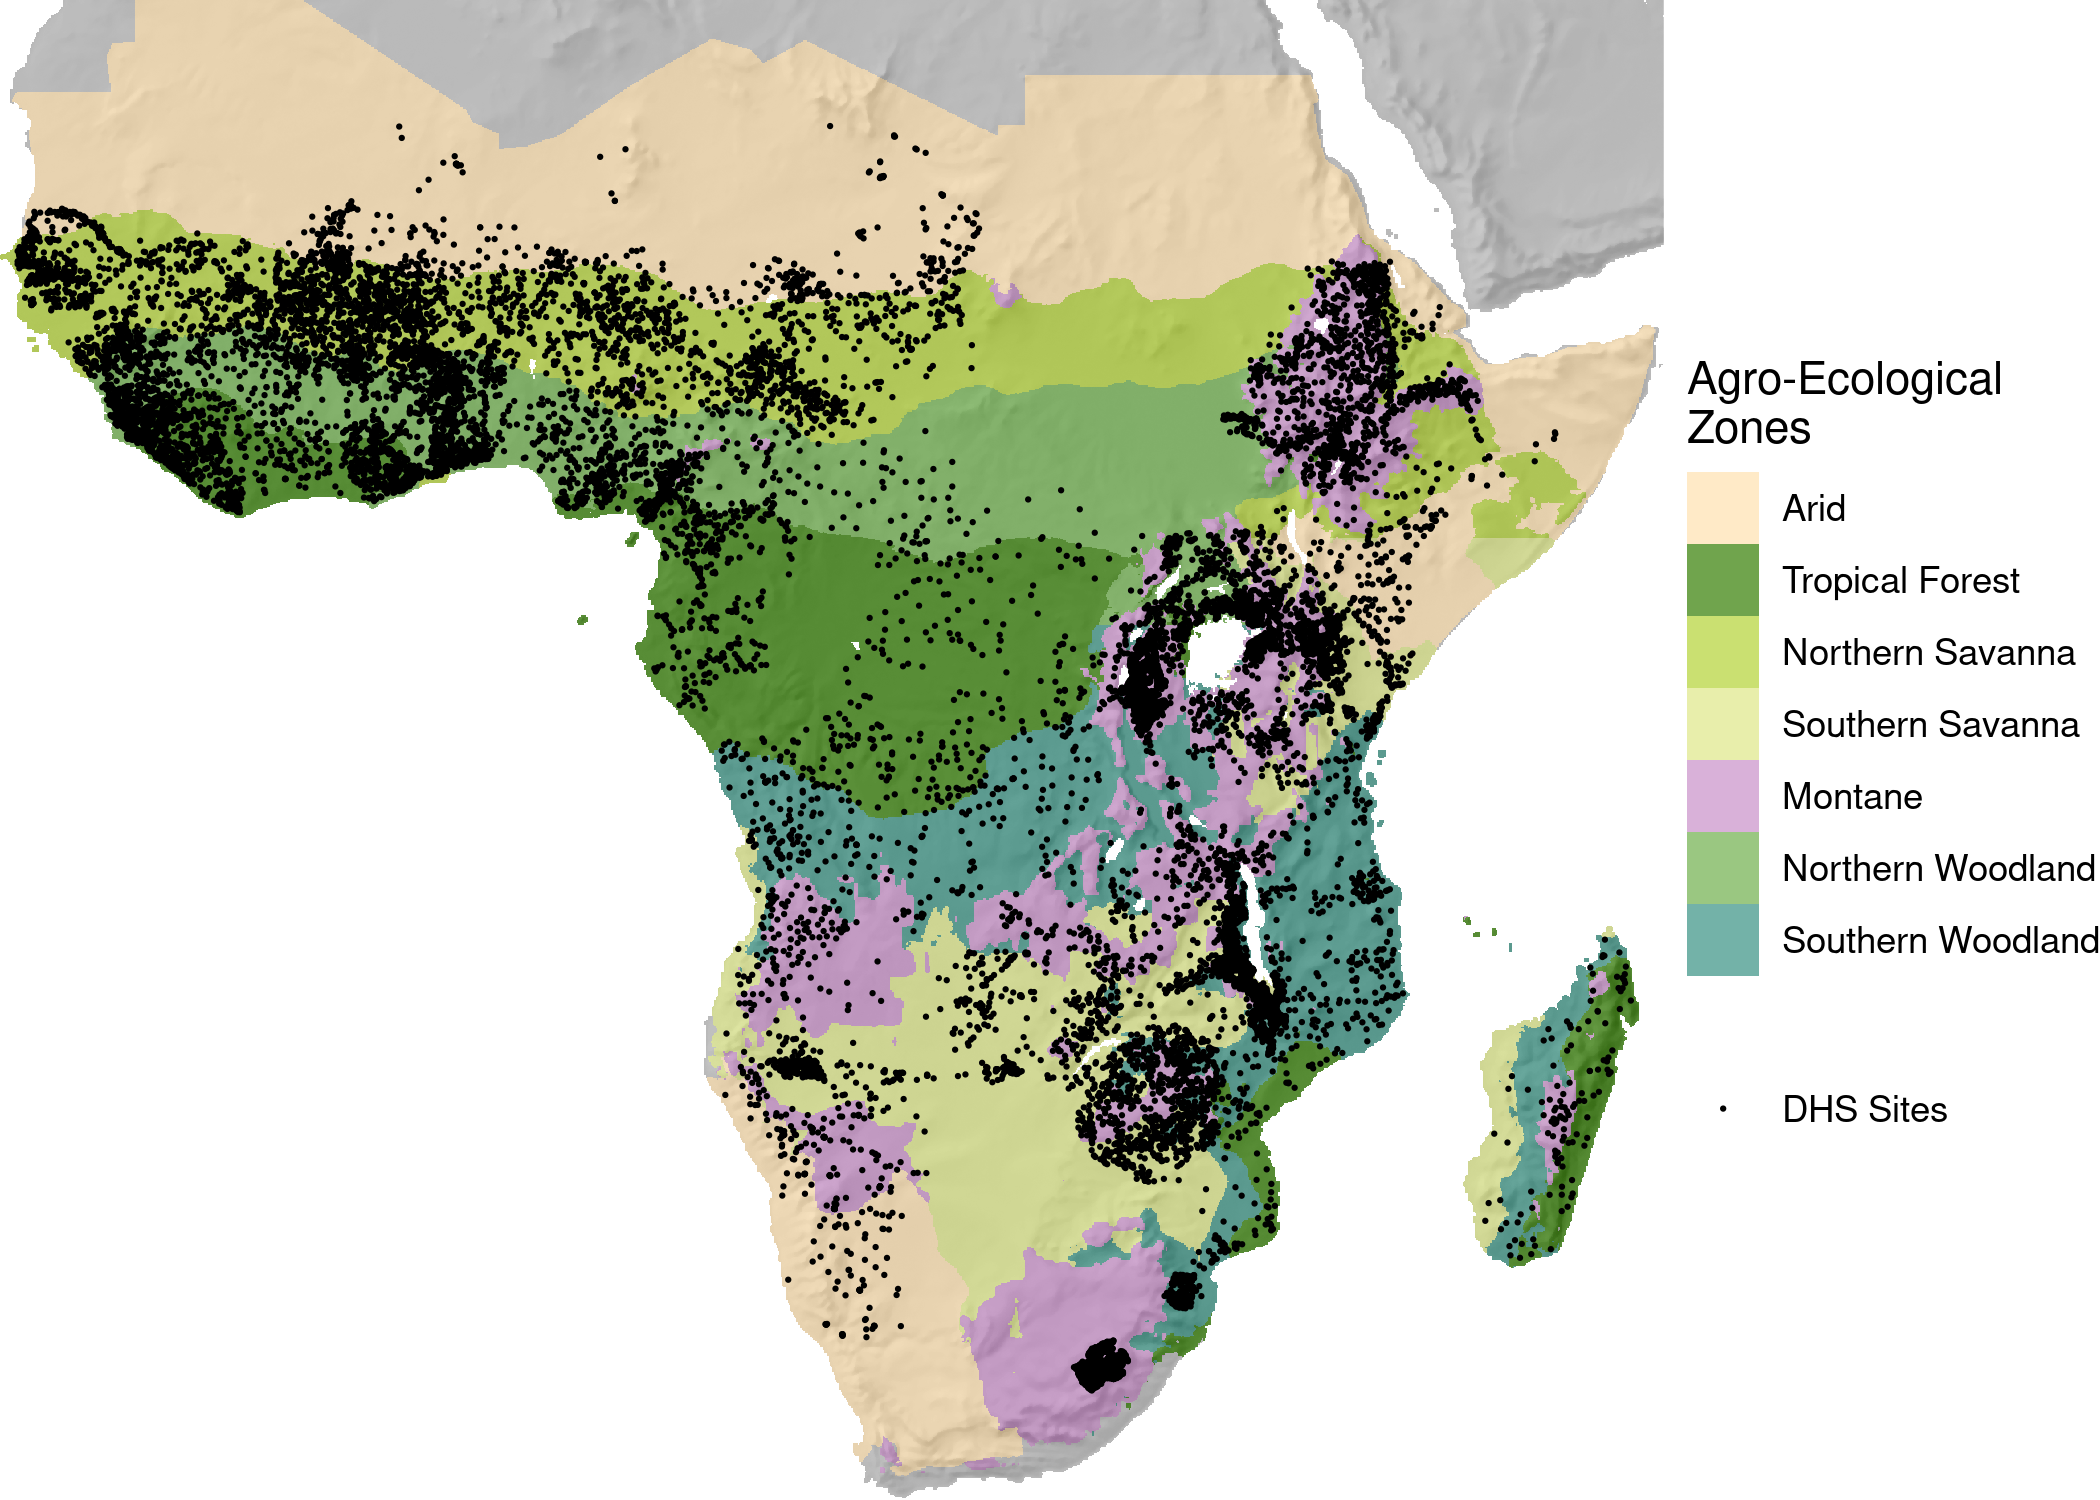
\includegraphics[width=0.8\linewidth]{AEZ_Sites.png}
	\caption{Agro-Ecological Zones and DHS sites included in the study.}
	\label{fig:AEZmap}
\end{figure}

Rainfall at 24 month SPEI, why??

Why "natural land cover"
	Raudsepp-Hearne
	Talk about african land ownership, quote that one person
	
	Can be a bigger refuge for the poor \& women
	Can provide a lot of other services
	
	scales, jittering, 25-km buffer
	

\section{Methods}
Controlling for endogeneity
	-matching
	-CBPS for GAMs

First test across the continent, then subset by AEZs

\section{Results}


\section{Discussion}

private agriculture vs commons

\section{Conclusion}


\bibliographystyle{apalike}
\bibliography{C://Users/matt/library}

\end{document}